\section{Applications of Integration}

\subsection{Average of a Function Over an Interval}
The average of a function over an interval is equal to the sum of all $y$ values divided by the length of the interval. The sum of all $y$ values is equivalent to the area under the curve, or the definite integral of the function over the interval. Therefore, the average of a function $f(x)$ for $a \leq x \leq b$ is:
\[ f_{avg} = \frac{1}{b - a} \int_a^b f(x) \; dx. \]

\subsection{Particle Motion (Position, Velocity and Acceleration)}
Similar to how derivatives can be used to get to velocity from position and acceleration from velocity, integrals can be used to go the other way around. That is,
\begin{align*}
    \int a(t) \; dt &= v(t) \\[5pt]
    \int v(t) \; dt &= p(t).
\end{align*}

There are three types of problems that involve velocity and position and require integrals to solve. They are described using point particles, but would work for any object. These are:
\begin{itemize}
    \item \textbf{Displacement:} the distance from a particle's starting position to its current position. If it moves forward then back again, displacement would not count the distance travelled back. The displacement from point $x = a$ to $x = b$ is given by:
    \[ \int_a^b v(x) \; dx. \]

    \item \textbf{Total distance:} the distance a particle has travelled to move between two points, including any back tracking. If a particle moves forward then back again, it would count the distance travelled back. The total distance travelled by a particle from point $x = a$ to $x = b$ is given by:
    \[ \int_a^b |v(x)| \; dx. \]

    \item \textbf{Actual position:} where the particle is at a specific time. The actual position of a particle at time $t = b$ is given by:
    \[ p(b) = p(a) + \int_a^b v(t) \; dt. \]
\end{itemize}

\noindent \textbf{Examples:}
\begin{enumerate}
    \item A particle with velocity $v(t) = 3\sqrt{t}$, moves in a straight line. How far does the particle move from $t = 1$ to $t = 4$?

	This problem is asking for the particle's total distance travelled, as hinted by ``how far does the particle move'' rather than ``how far is the particle from its starting position.'' Therefore, we can use the formula for total distance travelled.
    \begin{align*}
        d(t) &= \int_1^4 |3\sqrt{t}| \; dx \\[5pt]
        &= \left[ 2 t^{\frac{3}{2}} \right]_1^4 \\
        &= 16 - 2 \\
        d(t) &= 14
    \end{align*}

    The particle travels a total distance of $14$ units from $t = 1$ to $t = 3$.

    \item As a particle moves along the number line, its position, velocity and acceleration at time $t$ are given by $p(t)$, $v(t)$, and $a(t) = 12t - 4$, respectively. If $v(2) = 4$ and $s(0) = 1$, find $s(1)$.

    This question is asking for the actual position of the particle at $t = 1$, which can be found using the following formula:
    \[ s(1) = s(0) + \int_0^1 v(t) \; dt. \]

    However, to use this formula, we first need to find a particular solution for $v(t)$.
    \begin{align*}
        v(t) &= \int a(t) \; dt \\[5pt]
        &= \int 12t - 4 \; dt \\
        &= 6t^2 - 4t + C
    \end{align*}

    Solving for $C$:
    \begin{align*}
        v(2) &= 4 \\
        24 - 8 + C &= 4 \\
        C &= -12 \\
        v(t) &= 6t^2 - 4t - 12.
    \end{align*}

    Using this, we solve for the actual position of the particle:
    \begin{align*}
        s(1) &= s(0) + \int_0^1 v(t) \; dt \\[5pt]
        &= 1 + \int_0^1 6t^2 - 4t - 12 \; dt \\
        &= 1 + \left[ 2t^3 - 2t^2 - 12t \right]_0^1 \\
        &= 1 - 12 + 0 \\
        s(1) &= -11.
    \end{align*}

    Therefore, the position of the particle at $t = 1$ is $-11$ units.
\end{enumerate}

\subsection{Area Between Curves}

\subsubsection{Area Under a Single Curve}
The most basic type of area between curves is the area under a single curve. The area under the curve of function $f(x)$ over the interval $a \leq x \leq b$ is:
\[ \int_a^b f(x) \; dx. \]

\noindent \textbf{Examples:}
\begin{enumerate}
    \item What is the area under the curve of $\cos(x)$ from $0$ to $\frac{\pi}{2}$?

    This is found as follows:
    \begin{align*}
        \int_0^{\frac{\pi}{2}} \cos(x) \; dx &= \left[ \sin(x) \right]_0^{\frac{\pi}{2}} \\[5pt]
        &= 1 - 0 \\
        \int_0^{\frac{\pi}{2}} \cos(x) \; dx &= 1.
    \end{align*}

    This area is shown below.
    \begin{figure}[H]
        \centering
        \frame{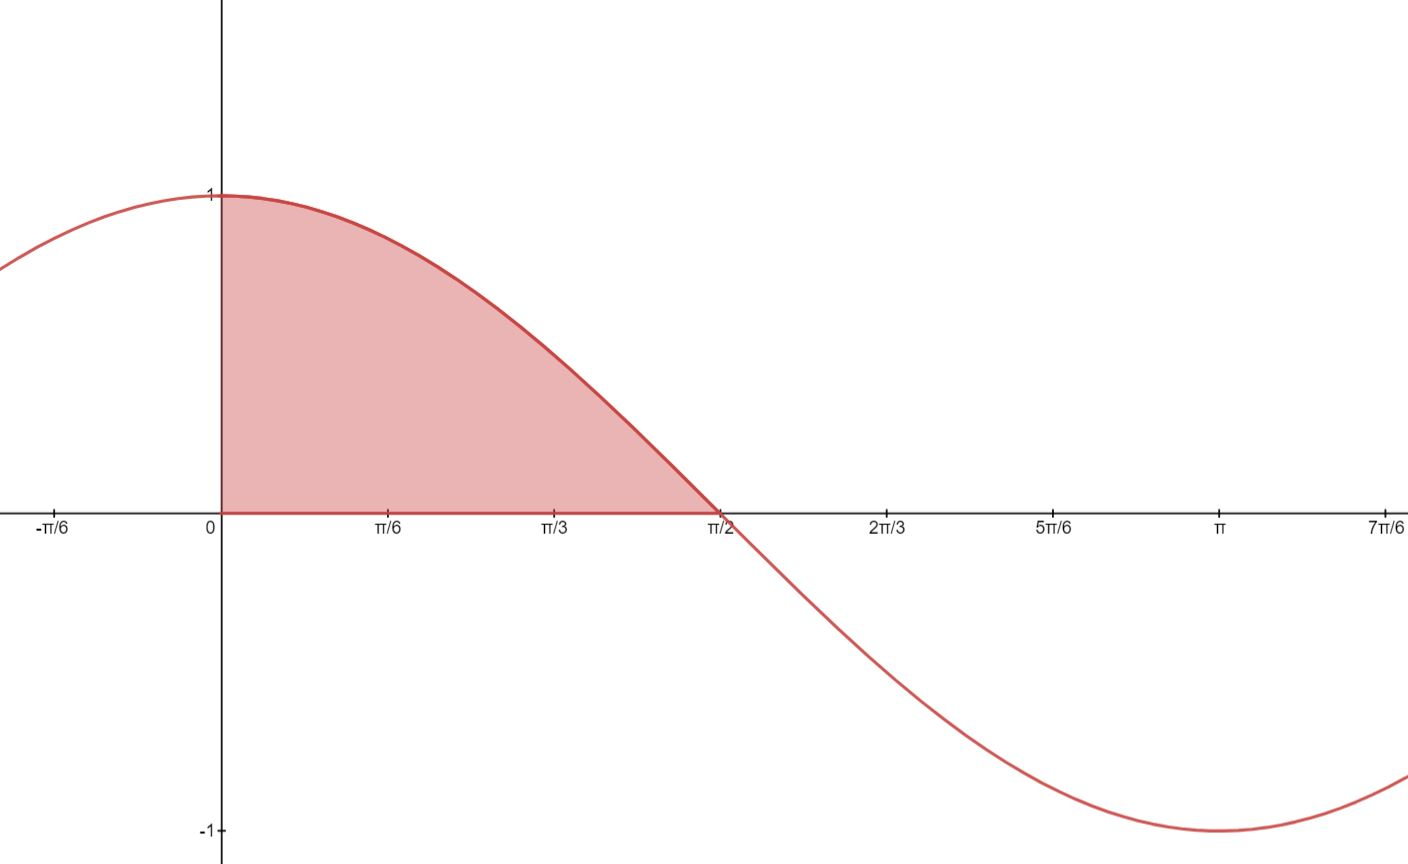
\includegraphics[width=0.4\textwidth]{images/fig15.JPG}}
        \caption{Area under $\cos(x)$ from $0$ to $\frac{\pi}{2}$.}
        \label{fig:area_cosx_pos}
    \end{figure}

    \item What is the area under the curve of $\cos(x)$ from $\frac{\pi}{2}$ to $\pi$?

    This is found as follows:
    \begin{align*}
        \int_{\frac{\pi}{2}}^\pi \cos(x) \; dx &= \left[ \sin(x) \right]_{\frac{\pi}{2}}^\pi \\[5pt]
        &= 0 - 1 \\
        \int_{\frac{\pi}{2}}^\pi \cos(x) \; dx &= -1.
    \end{align*}

    Note that this area is negative because it is under the $x$-axis. This is shown below.
    \begin{figure}[H]
        \centering
        \frame{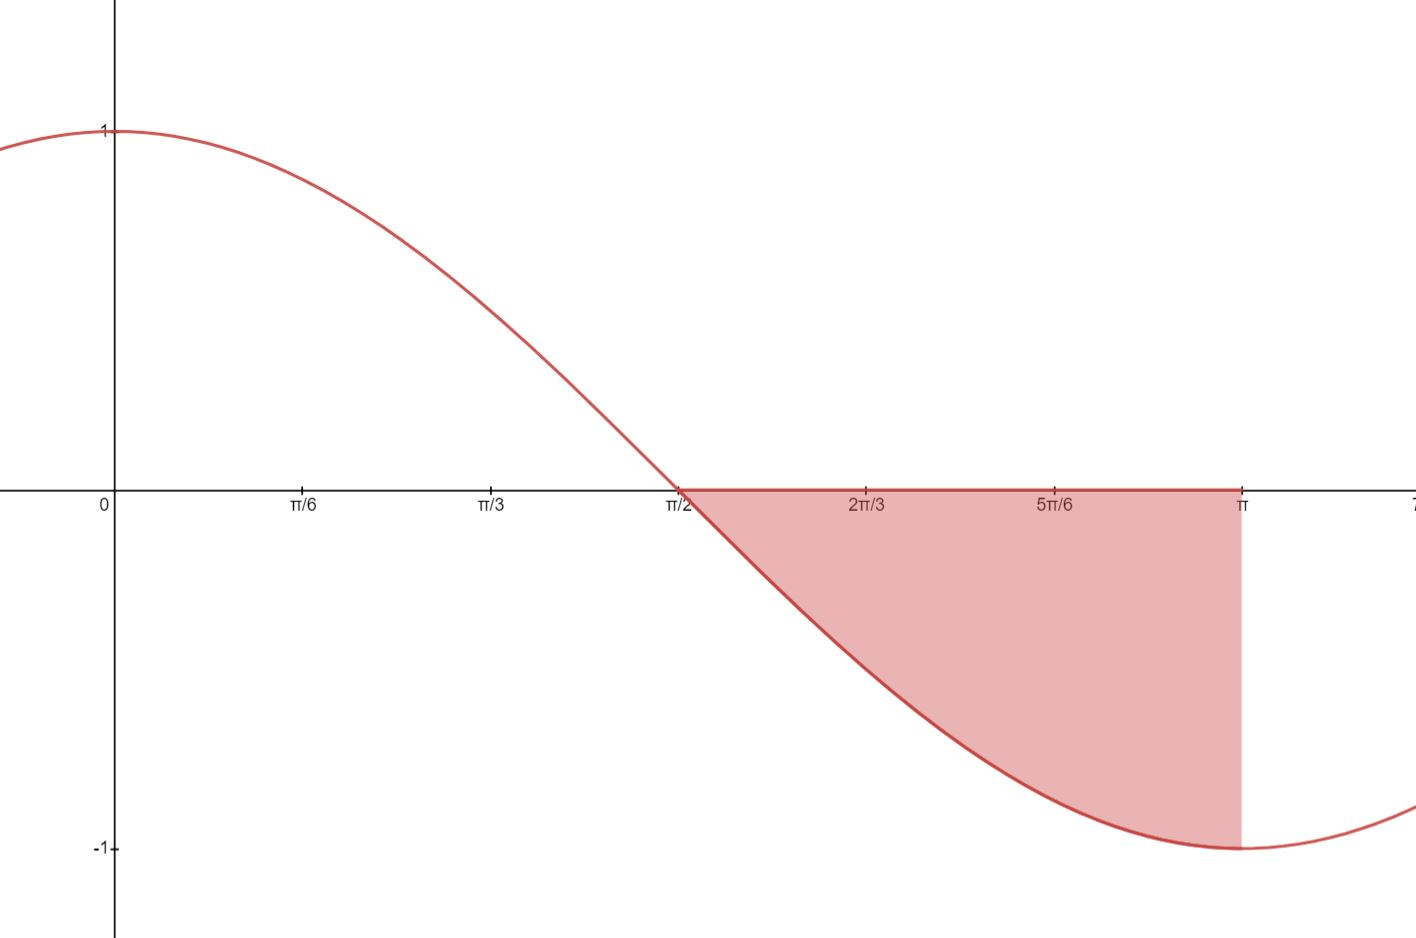
\includegraphics[width=0.4\textwidth]{images/fig16.JPG}}
        \caption{Area under $\cos(x)$ from $\frac{\pi}{2}$ to $\pi$.}
        \label{fig:area_cosx_neg}
    \end{figure}
\end{enumerate}

\subsubsection{Curves as Functions of x}
% mention the absolute value method:
% \int |f(x)| dx

\subsubsection{Curves as Functions of y}

\subsection{Volumes with Cross-Sections}

\subsubsection{Square and Rectangle Cross-Sections}

\subsubsection{Disc Method}

\subsubsection{Washer Method}

\subsection{Determining the Length of a Planar Curve}
